\capitulo{2}{Introducción}
% Se pueden añadir todas las subsecciones que queramos o necesitemos.

Descripción del contenido del trabajo y de la estructura de la memoria y del resto de materiales entregados.


\section{Conceptos teóricos básicos.} %Explicación de los conceptos teóricos básicos necesarios para que cualquier miembro del tribunal pueda entender el trabajo realizado.
Para llevar a cabo este trabajo hay que comprender su base, en este caso el control postural, qué es, su importancia y todo lo que ello conlleva.\cite{wiki:latex} % Citar el librio

Antes de comenzar se deben conocer los siguientes conceptos básicos y componentes que engloban el control postural:

\begin{itemize}
    \item Centro de masas o CDM que es la media de todos los centros de masas de las distintas partes del cuerpo, es responsable del equilibrio.
    \item Centro de presiones o CDP es la proyección sobre la base de sustentación del centro de masas del cuerpo.
    \item Centro de gravedad o CDG es el punto del cuerpo donde se concentra la fuerza de gravedad.
    \item Área de apoyo es el área sobre la que el cuerpo descarga su peso de forma efectiva.
    \item Base de sustentación que es la superficie disponible sobre la que un cuerpo puede apoyar su peso.
    \item Límite de estabilidad es el trayecto por el cual una persona puede realizar un movimiento sin perder su equilibrio y poder realizar ajustes posturales, este límite no es fijo, depende del tiempo, de la tarea o del entorno.
    \item Postura es la orientación y el alineamiento del cuerpo respecto al entorno.
    \item Orientación postural es la capacidad de mantener la relación entre las distintas partes del cuerpo y el entorno para realizar una actividad.
    \item Sinergia postural es la relación entre la contracción muscular y las rotaciones articulares para estabilizar la postura.
    \item Balanceo postural es el desplazamiento constante y la corrección del centro de gravedad para mantener la postura.
\end{itemize}

La postura nace de la relación entre el entorno, el individuo y la actividad que debe realizar. Y, por tanto, el control postural es el control de la posición corporal en el espacio con el fin de obtener la estabilidad, y la orientación que necesitamos para poder realizar las actividades diarias, su profesión o aficiones. La estabilidad se define como la capacidad de mantener la proyección del centro de gravedad dentro de una base de sustentación, mientras que la orientación es la capacidad de mantener la relación adecuada entre las distintas partes del cuerpo al realizar una tarea teniendo en cuenta el entorno.

Para poder cumplir con el objetivo del control postural el cuerpo tiene que anticiparse, mantenerse y reaccionar. El control postural requiere que interaccionen distintos sistemas del cuerpo para abarcar la estabilidad, la percepción de la orientación espacial, el alineamiento del cuerpo, la lucha contra la gravedad al realizar un movimiento y la respuesta a posibles perturbaciones de origen sensorial o mecánico.

Principalmente en el control postural interviene el sistema nervioso, como centro de control, manteniendo la postura y el equilibrio gracias a la recogida e interpretación de información de los receptores y a la producción de órdenes; y, el sistema musculoesquelético, ya que se requiere de una musculatura capaz de adaptarse a los cambios. Además, se utilizan experiencias previas para elaborar el esquema corporal.

Por todo ello se va a conocer la relación del sistema nervioso y la postura, algunas estrategias del control postural y su importancia o desarrollo.

%Subseccion
\subsection{El sistema nervioso y la postura.} 
El sistema nervioso se compone de diferentes estructuras como son las neuronas o las células de neuroglia que se encargan de mantener la homeostasis corporal regulando y coordinando las distintas funciones del organismo.

Asimismo, el sistema nervioso se puede dividir en sistema nervioso central que se encuentra compuesto por la médula espinal y el encéfalo, y el sistema nervioso periférico que está compuesto por ganglios y nervios.

El sistema nervioso también se puede dividir en función del tipo de respuestas de las que se encargan, si se encarga de las respuestas involuntarios se trata del sistema nervioso autónomo que, a su vez, se divide en los sistemas simpático y parasimpático. En el caso de las respuestas voluntarias del organismo se llama sistema nervioso somático.

Los receptores son los que se encargan de recoger la información que recibe el sistema nervioso mediante mecanismos de retroalimentación, estos elementos se encuentran en los músculos, para poder detectar el movimiento. Por otra parte, se necesita también la información recogida por la vista, el sistema vestibular del oído interno o las señales procedentes de las modificaciones de presión.

Si en algún caso se producen perturbaciones los receptores detectarán esos imprevistos y proporcionarán información acerca de las nuevas condiciones para así adaptar el tono postural. Por ejemplo si los receptores de presión de los pies registran el desplazamiento mínimo durante la bipedestación y se transmite la información por el nervio periférico, seguido de la medula espinal, el tracto espinocerebeloso y desde el cerebelo a la formación reticular y a los núcleos vestibulares. Si se desplaza la cabeza se crea una aceleración en dirección anterior que se registra y se transmite esa información a los núcleos vestibulares. 

Las reacciones de equilibrio son la respuesta al control postural, los núcleos vestibulares activan la musculatura de la core-stability que está formada por los músculos del suelo pélvico, los músculos profundos paravertebrales y sacrolumbares, y, la musculatura abdominal y lateral. En función del tipo de desplazamiento se activarán una cadena u otra, ya sean la cadena anterior, la posterior, la lateral o combinaciones de las mismas.

\subsection{Estrategias de control postural.} 
El control postural y sus ajustes se dan en tronco, tobillos y caderas, para así mantener el equilibrio, creando la estabilidad que permite los movimientos al realizar distintas actividades.

Existe un modelo que define 3 elementos que modifican, construyen y mantienen la postura, el modelo de sistemas dinámicos de Bernstein. Lo elementos en cuestión son los factores individuales, la tarea a realizar y el entorno. 

Los factores individuales son aquellos pertenecientes a cada individuo, pueden variar su influencia con entrenamiento. Dentro de los factores individuales encontramos los elementos sensitivos que dan información respecto al movimiento y la posición del centro de gravedad e incluyen las aferencias visuales (posición respecto al entorno), el sistema somatosensitivo (son los receptores de los músculos, la piel u otros tejidos, dan información acerca de las variaciones de la orientación postural) y el vestibular (es básicamente el oído, posición de la cabeza); también encontramos los elementos motores que hacen referencia a las exigencias musculoesqueléticas (fuerza, flexibilidad o alineación de las partes del cuerpo) y neuromusculares (patrones de movimiento y contracción de los músculos)  necesarias para el ajuste postural; y, los elementos cognitivos que refieren a las necesidades psicológicas y cognitivas relacionadas con la actitud postural.

Igualmente, existen diferentes estrategias de control de la postura, como aquellas que se centran en el equilibrio, controlando las oscilaciones o balanceos espontáneos. Algunas de estas estrategias son las de controlar la correcta alineación corporal, minimizando las fuerzas gravitatorias; el suficiente tono muscular mediante el control de la resistencia de un músculo a ser estirado; el correcto tono postural, a partir del control de la fuerza de gravedad; o, el control de las reacciones posturales o de balance mediante ajustes compuestos de reacciones de equilibrio, enderezamiento y de apoyo. 

Por otro lado, la memoria implícita que se da en el cerebelo y en los núcleos basales proporciona información sobre dónde, cuánto y cómo se debe ajustar el tono postural para compensar los desplazamientos.

Otras estrategias para mantener el control postural son las que describen Shumway-Cook y Woollacott, la ‘ankle strategy’ que se basa en la bipedestación mantenida por la base de sustentación pequeña que serán los tobillos, la ‘hip strategy’ que se basa en controlar los centros de masas en un desplazamiento de peso mayor y la ‘stepping strateging’ que se basa en una base de sustentación aún mayor.

\subsection{Desarrollo del control postural.} 
Las necesidades de estabilidad cambian con la tarea que se debe realizar. El desarrollo de control postural en niños se produce en tres etapas, primero, se debe desarrollar el control encefálico, después la sedestación (capacidad de sentarse) y, por último, la bipedestación.

Además, la postura y el equilibrio varían con la edad, por una parte, los niños pequeños no tienen suficientemente desarrollado las aferencias sensoriales, y por otra los adultos mayores presentan involución cognitiva de sus estructuras cerebrales, todos ellos ven disminuido el control postural.

Asimismo, pacientes con traumatismos craneoencefálico, esclerosis múltiple, infartos u otras lesiones en el sistema nervioso central pueden tener afectado alguno de elementos implicados en el control de la postura y por lo que su control postural se verá afectado. En algunos casos también influyen los factores psicológicos, una persona con depresión o un problema de atención también puede llegar a influir sobre ese control postural.


%Sub-subseccion
\subsubsection{Sub Subsección}

\subsubsection{Sub Subsección}

En esta sección y el resto de secciones de la memoria puede ser necesario incluir listas de items.

% Listas de puntos 
\begin{itemize}
    \item item1
    \item item2
    \item item3
\end{itemize}

Listas enumeradas.
% Enumeraciones
\begin{enumerate}
    \item item1
    \item item2
    \item item3
\end{enumerate}

Figuras, como la figura \ref{fig:escudo} que aparece en la página \pageref{fig:escudo}. 

Puedes aprender más de las figuras en la dirección \url{https://es.overleaf.com/learn/latex/Inserting_Images} % más informacion de como utilizar figuras

% Inicio de la figura
\begin{figure}[h]
    \centering
    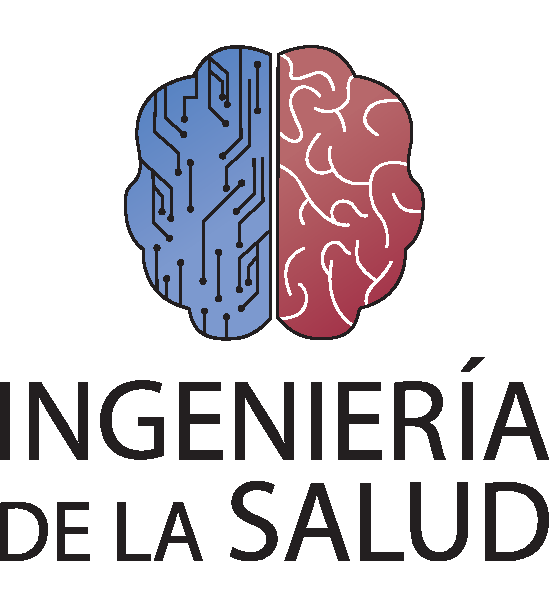
\includegraphics[width=0.25\textwidth]{img/escudoSalud.pdf}
    \caption{Pie de la figura}
    \label{fig:escudo} % Esta etiqueta es la que permite que se encuentr referenciada en el texto (es muy importante que siempre estén referenciadas en el texto)
\end{figure}


También se pueden insertar tablas como \ref{tab:my-table}, que ha sido generada con \url{https://www.tablesgenerator.com/}. % Este enlace permite crear tablas y te genera el código latex

% Ejemplos de tablas
\begin{table}[]
\begin{tabular}{lll}
a & b & c \\
1 & 2 & 3 \\
4 & 5 & 6
\end{tabular}
\caption{}
\label{tab:my-table}
\end{table}

Es necesario que todas las figuras y tablas aparezca referenciadas en el texto, como estos ejemplos.

Todos los conceptos teóricos deben de estar correctamente referenciados en la bibliografía. Por ejemplo, aquí estoy citando la página de \LaTeX{} de Wikipedia \cite{wiki:latex}. %El comando \cite permite referenciar las citas bibliográficas, siempre se tienen que referenciar las citas de la bibliografía.

También puede ser necesario utilizar notas al pie \footnote{como por ejemplo esta}, para aclarar algunos conceptos.


\section{Estado del arte y trabajos relacionados.}

\begin{comment}
Revisión bibliografica de que se está haciendo en la industria o la academia relativo al problema que se está tratando.

Enumeración y resumen de todos los trabajos relacionados de interés.


También se puede incluir que existen gran variedad de dispositivos cuyo fin es el de medir o controlar la postura.
\end{comment}
En la actualidad existen multitud de dispositivos electrónicos compuestos de sensores, actuadores y algoritmo cuya finalidad es algún tipo de control postural, ya sea regulándola o modificando la postura. Existen diferentes aplicaciones: 
\begin{itemize}
    \item Mejora de la estabilidad del equilibrio de las personas con alguna alteración en el control postural como pueden ser personas con parálisis cerebral, esclerosis múltiple, Párkinson… 

    \item Prevención de una mala postura en personas que están sentadas o realizando alguna actividad. 

    \item Monitorización de la postura como feedback para mejora de ergonomía en diferentes personas por ejemplo en atletas. 
\end{itemize}

Se necesita conocer las especificaciones que requerirán los dispositivos en función de la aplicación a la que se encuentren destinados. Algunas especificaciones que se deben tener en cuenta al diseñar o elegir un dispositivo electrónico de control postural son: 
\begin{itemize}
    \item Precisión y fiabilidad de los sensores y actuadores para detectar y responder correctamente a los cambios en la postura. 

    \item Facilidad de uso y comodidad, para que se adapte a las necesidades del usuario y a su actividad. 

    \item Autonomía y conectividad del dispositivo para que se adapte a las actividades que realiza el usuario. 
\end{itemize}

Por todo ello se realiza un estudio de distintos dispositivos que existen en la actualidad cuya finalidad u funcionamiento es similar al objetivo de este proyecto. 


